\documentclass[a4paper,12pt]{article}
\usepackage[a4paper,top=1.3cm,bottom=2cm,left=1.5cm,right=1.5cm,marginparwidth=0.75cm]{geometry}
%%% Работа с русским языком
\usepackage{cmap}					% поиск в PDF
\usepackage{mathtext} 				% русские буквы в фомулах
\usepackage[T2A]{fontenc}			% кодировка
\usepackage[utf8]{inputenc}			% кодировка исходного текста
\usepackage[english,russian]{babel}	% локализация и переносы

\usepackage{graphicx}
\usepackage{mathtools}
\usepackage{wrapfig}
\usepackage{tabularx}
\usepackage{amssymb}
\usepackage{hyperref}
\usepackage[rgb]{xcolor}
\hypersetup{colorlinks=true,urlcolor=blue}
\setcounter{secnumdepth}{0}
%% Шрифты
\usepackage{euscript}	 % Шрифт Евклид
\usepackage{amsmath}
\usepackage{mathtools}
%%% Заголовок
\author{Tsvetkova Amelia}
\title{Лабораторная работа по общей физике}

\date{\today}
\begin{document}
\begin{titlepage}
    \newpage
    \begin{center}
    {\large МОСКОВСКИЙ ФИЗИКО-ТЕХНИЧЕСКИЙ ИНСТИТУТ (НАЦИОНАЛЬНЫЙ ИССЛЕДОВАТЕЛЬСКИЙ УНИВЕРСИТЕТ)}
    \vspace{1cm}

    {\largeФизтех-школа аэрокосмических технологий}
    \vspace{6em}
    \end{center}
    
    \vspace{1.2em}

    \begin{center}
    \Large Лабораторная работа №4.7.3 \\
    Изучение поляризованного света
    \linebreak
    \end{center}
    
    \vspace{11em}
    
    \begin{flushright}
                       {\large Работу выполнила\\
                       Цветкова Амелия Антоновна\\
                       Б03-303 }
    \end{flushright}

    \vspace{\fill}

    \begin{center}
    Долгопрудный, 2025
    \end{center}

    \end{titlepage}

\paragraph{Цель работы:} ознакомление с методами получения и анализа поляризованного света.

\paragraph{В работе используются:} оптическая скамья с осветителем; зеленый светофильтр; два поляроида; черное зеркало; полированная эбонитовая пластинка в одну длину волны для зеленого света (пластинка чувствительного оттенка).

\section{Теоретические сведения}

\subsection{Типы поляризации, основные понятия}
\textit{Плоскостью поляризации} наз. плоскость построенная на векторах ($\mathbf{E}$, $\mathbf{k}$). Плоская волна наз. \textit{линейно поляризованной}, если ориентация плоскости поляризации не меняется во времени. В \textit{естественном} свете плоскость поляризации меняется случайным образом.

Плоские электромагнитные волны являются поперечными, т.е. проекции осциллирующих электрического и магнитного полей на направление распространения такой волны равны нулю. По теореме Гаусса:
$$
\text{div}\vec{E}=\frac{\partial E_x}{\partial x}+\frac{\partial E_y}{\partial y}+\frac{\partial E_z}{\partial z}=0
$$

Из уравнения циркуляции магнитного поля:
$$
(\text{rot}\vec{H})_z=\frac{\partial H_y}{\partial x}+\frac{\partial H_x}{\partial y}+\frac{1}{c}\frac{\partial E_z}{\partial t}
$$

В итоге получаем уравнения:
$$
\left\{ 
\begin{array}{ll} 
(\text{rot}\vec{E})_y=\frac{\partial E_x}{\partial z}=-\frac{1}{c}\frac{\partial H_y}{\partial t}, \\
(\text{rot}\vec{H})_x=-\frac{\partial H_y}{\partial z}=\frac{1}{c}\frac{\partial E_x}{\partial t}\end{array}\right.
$$
и
$$
\left\{ 
\begin{array}{ll} 
(\text{rot}\vec{E})_x=\frac{\partial E_y}{\partial z}=\frac{1}{c}\frac{\partial H_x}{\partial t}, \\
(\text{rot}\vec{H})_y=\frac{\partial H_x}{\partial z}=\frac{1}{c}\frac{\partial E_y}{\partial t}\end{array}\right.
$$

В любой точке пространства концы векторов $\vec{E}$ и $\vec{H}$ в каждой из этих волн движутся по отрезкам прямых линий в плокости $(E_x, E_y)$, поэтому они \texttt{линейно поляризованными}.

Если обе описанные выше монохроматические волны распространяются одновременно, то концы векторов $\vec{E}$ и $\vec{H}$ движутся по эллипсам в плоскости $(E_x, E_y)$. Это наиболее общий тип поляризации - \texttt{эллиптическая поляризация}. Если полуоси эллипса равны, то таккую поляризацию наз. \texttt{круговой}. Свет наз. правополяризованным, если для наблюдателя, смотрящего навстречу лучу, вектор $\vec{E}$ вращается по часовой стрелке. 

Свет с круговой поляризацией можно представить как суперпозицию двух линейно поляризованных волн:
$$
\mathbf{E} = \mathbf{E}_x +\mathbf{E}_y, \quad \mathbf{E}_x = \mathbf{e}_xE_0\cos(wt), \quad \mathbf{E}_y = \mathbf{e}_yE_0\sin(wt)
$$

Монохроматические волны всегда являются так или иначе поляризованными. Если же свет квазимонохроматический (обладает нулевой шириной спектра), то возможны три случая. В первом поляризация не меняется от цуга к цугу, несмотря на сбой фазы между ними. Такой свет считается поляризованным наравне с монохроматическим. Во втором поляризации цугов меняются случайным и независимым образом. Такой свет считают неполяризованным. И в третьем случае поляризации цугов отличаются, но некоторые поляризации появляются с большей вероятностью, чем другие. Такой свет считается поляризованным частично, его можно рассматривать как смесь поляризованного и неполяризованного света.

\subsection{Получение поляризованного света}

Устройства, с помощью которых из естественного света получают поляризованный, наз. поляризаторами. Они разделяют исходный пучок на две компоненты, ортогональные по типу поляризации, одну из них пропускают, а другую поглощают или отклоняют. Действие их может быть основано на одном из четырех явлений: дихроизме, двойном лучепреломлении в кристаллах, отражении и преломлении на границе изотропных диэлектриков и поляризации при рассеянии света.

\texttt{Дихроизм} (анизотропия поглощения) - это способность вещества поглощать свет по-разному в зависимости от его поляризации. 

\texttt{Двойное лучепреломление} в анизотропнных кристаллах - результат зависимости в этих кристаллах кожффициента преломления от поляризации световой волны.

\texttt{Поляризация света при отражении и преломлении} на границе изотропного диэлетрика следует из формул Френеля.
$$
\rho_\perp=\frac{\sin^2{(\varphi-r)}}{\sin^2{(\varphi+r)}}, \quad \rho_\|=\frac{\tan^2{(\varphi-r)}}{\tan^2{(\varphi+r)}}
$$
здесь $\varphi$ - угол падения, а $r$ - угол преломления волны. Отсюда следует, что $\varphi+r=90^\circ$, т.е. угол между направлениями распространения отраженной и преломленной волн является прямым, коэффициент отражения $\rho_\|$ обращается в ноль и отраженный свет оказывается полностью поляризованным. Соотвествующий угол падения
$$
\varphi_\text{Б} =\arctan{(n)}
$$
где $n$ - коэффициент преломления среды, наз. углом \texttt{Брюстера} или углом полной поляризации. 

При \texttt{рассеянии} света на частицах пыли, молекулах газа и даже на атомах в кристаллах рассеянная волна также оказывается поляризованной, причем преимущественное направление электрических колебаний перпендикулярно падающему лучу. Интенсивность рассеянного света в газах невелика, причем согласно закон Релея она пропорциональна $1/\lambda^4$.

\subsection{Наблюдение и анализ поляризованного света. Закон Малюса}

Для анализа поляризованного света его пропускают через поляризатор, который в этом случае принято называть анализаторами. При прохождении через анализатор линейно поляризованного света интенсивность прошедшей волны пропорциональна квадрату проекции амплитуды исходной волны на разрешенное направление поляризатора, т.е.
$$
I=I_0\cos^2{\varphi},
$$
где $\varphi$ - угол между направлением электрических колебаний анализируемой волны и разрешенным направлением поляризатора. 

Для частично линейно поляризованного света вводят понятие \texttt{степени поляризации}
$$
P=\frac{I_{max}-I_{min}}{I_{max}+I_{min}},
$$
где $I_{max}$ и $I_{min}$ - соответственно максимальное и минимальное значения интенсивности света, прошедшего через анализатор при различных углах $\varphi$.

\subsection{Двойное лучепреломление}

В некоторых кристаллах потенциальные ямы, в которых находятся электроны вблизи углов решетки, не являются сферически-симметричными. При этом систему координат всегда возможно выбрать так, что для малых отклонений от положения равновесия потенциальная энергия электронов будет иметь вид 
$$
U=a_xx^2+a_yy^2+a_zz^2
$$

Если все три коэффициента $a_x, a_y, a_z$ различны, то кристалл наз. двуосным, если два коэффициента равны - одноосным. Положим $a_y=a_z=a_\perp, a_x=a_\|$. Ось $x$ при этом наз. \texttt{оптической осью кристалла}. 

\subsection{Определение направления разрешенной плоскости колебаний поляроида}

Определить направление разрешенных колебаний поляроида можно с помощью черного зеркала.

При падении света на отражающую поверхность под углом Брюстера, свет в отраженном луче почти полностью поляризован, а вектор $\vec{E}$ параллелен отражающей поверхности. Луч света, прошедший поляроид и отразившийся от черного зеркала, имеет минимальную интенсивность при выполнении двух условий: во-первых, свет падает на отражающую поверхность под углом Брюстера, во-вторых, в падающем пучке вектор $\vec{E}$ лежит в плоскости падения.

Вращая поляроид вокруг направления луча и черное зеркало вокруг оси, перпендикулярной лучу, методом последовательных приближений можно добиться минимальной яркости луча, отраженного от зеркала и определить разрешенное направление поляроида.

Измеряя угол поворота зеркала, можно определить коэффициент преломления материала, из которого изготовлено зеркало.

\subsection{Получение эллиптически поляризованного света}

Эллиптически поляризованный свет можно получить из линейно поляризованного с помощью двоякопреломляющих кристаллических пластинок.

\begin{figure}[h]
\centering
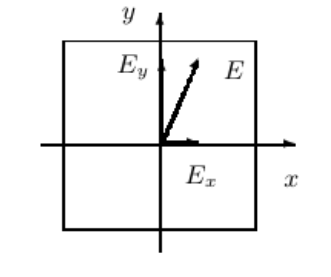
\includegraphics[width=0.2\linewidth]{img1.png}
\caption{Разложение линейно поляризованного света по главным направлениям двоякопреломляющей пластинки}
\label{img1}
\end{figure}

Двоякопреломляющая пластинка имеет два взаимно перпендикулярных главных направления, совпадающих с осями эллипсоида диэлектрической проницаемости. Волны, поляризоваанные вдоль главных направлений, распространяются в пластинке с разными скоростями, не изменяя харакетра своей поляризации. Эти волны наз. \textit{главными}. Мы будем обозначать показатели преломления для главных волн через $n_x$ и $n_y$, где $x$ и $y$ - главные направления кристаллической пластинки.

Пусть на пластинку падает линейно поляризованная волна, электрический вектор которой ориентирован под некоторым углом $\alpha$ к оси $x$. Разложим вектор $\vec{E}$ на составляющие $E_x$ и $E_y$. На входе пластинки $E_x$ и $E_y$ находятся в фазе. На выхожде из-за разности скоростей между ними появляется разность хода $d(n_x-n_y)$, при этом сдвиг фаз определяется соотношением:
\begin{equation}
    \Delta\varphi=\frac{2\pi}{m}=kd(n_x-n_y)
\end{equation}
где $k$ - волновое число, $d$- толщина кристаллической пластинки. При сложении двух взаимно перпендикулярных колебаний, обладающих некоторым сдвигом фаз, образуется колебание, поляризованное по эллипсу.

Рассмотрим частные случаи:
\begin{enumerate}
    \item Пластинка дает сдвиг фаз $2\pi$. В результатте сложения волн на выходе пластинки образуется линейно поляризованная волна с тем же направлением колебаний, что и в падающей волне.
    \begin{figure}[h]
    \centering
    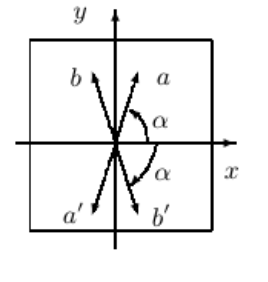
\includegraphics[width=0.2\linewidth]{img2.png}
    \caption{Поворот направления колебаний с помощью пластинки в $\lambda/2$}
    \label{img2}
    \end{figure}
    \item Пластинка дает сдвиг фаз $\pi$. На выходе пластинки снова образуется линейно поляризованная волна. Напраление $bb'$ колебаний этой волны повернуто относительно направления $aa'$ колебаний падающей волны. Направление $bb'$ является зеркальным отображением направления $aa'$ относительно одного из главных направлений пластинки. Такую пластинку используют для поворота направления колебаний линейно поляризованного света.
    \item Пластинка создает между колебаниями сдвиг фаз $\pi/2$. При сложении двух взаимно перпендикулярных колебаний, имеющих разность фаз $\pi/2$, образуется эллипс, главные оси которого совпадают с координатными осями $x$ и $y$. При равенстве амплитуд $E_x^{max}=E_y^{max}$ возникает круговая поляризация.
\end{enumerate}

\subsection{Анализ эллиптически поляризованного света}

Анализ эллиптически поляризованного света сводится к нахождению гланых осей эллипса поляризации и к определению направления вращения электрического вектора.

Главные оси эллипса поляризации определяются с помощью анализатора по максимуму и минимуум интенсивности проходящего света. Направление вращения электрического вектора может быть найдено с помощью пластинки в четверть длины волны, для которой известно, какая из главных волн, $E_x$ или $E_y$, имеет большую скорость распространения.

Выберем для определенности координатные оси $x$ и $y$ на пластинке так, чтобы $n_x<n_y$. В этом случае главная волна $E_x$ имеет большую скорость распространения. Поместим такую пластинку на пути эллиптически поляризованного света и совместим главные направления пластинки $\lambda/4$ с главными осями эллипса поляризации. На выходе их этой пластинки сдвиг фаз между $E_x$ и $E_y$ вместо $\pi/2$ станет равным 0 или $\pi$. Свет откажется линейно поляризованным. Из двух возможных значений сдвига фаз реализуется одно: то, которое соотвествует имеющемуся в волне направлению вращения электрического вектора.

Рассмотрим случай, когда электрический вектор в эллиптиически поляризованной волне вращается против часовой стрелки, если смотреть навстречу лучу. В этом случае, в волне, падающей на пластинку в $\lambda/4$, колебание $E_y$ отстает по фазе нан $\pi/2$ от колебания $E_x$. При прохождении через пластинку разность фаз увеличивается до $\pi$. На выходе из пластинки возникают линейно поляризованные волны со сдвигом фаз $\pi$. Сложение этих волн дает плоскопараллельную волну, электрический вектор которой располагается во втором и четвертом квадрантах координатной системы $x,y$.

Аналогично найдем, что при вращении электрического вектора по часовой стрелке направление колебаний в линейно поляризованной волне, выходящей из пластинки, располагается в первом и третьем квадрантах. Определяя направление колебаний на выходе из пластинки с помощью поляроида, можно определить характер эллиптичееской поляризации.

\subsection{Пластинка чувствительного оттенка}

Выше предполагалось известным, какому из двух направлений пластинки в четверть длины волны соответствует большая скорость распространения света. Установить это можно с помощью пластинки \textit{чувствительного оттенка} (так называют пластинку в $\lambda$ для зеленой спектральной компоненты, $\lambda=560$нм). Пластинка имеет форму стрелы, вдоль оси которой расположено главное направление, соответствующее большей скорости распространения.

\begin{figure}[h]
\centering
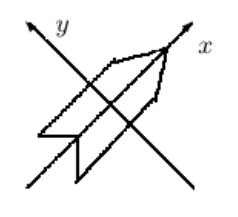
\includegraphics[width=0.2\linewidth]{img3.png}
\caption{Пластинка чувствительного оттенка}
\label{img3}
\end{figure}

Если эта пластинка помещена между скрещенными поляроидами и главные направления пластинки не параллельны направлениям разрешенных колебаний поляроидов, то при освещении белым светом пластинка кажется окрашенной в лилово-красный цвет. 

Если между скрещенными поляроидами поместить пластинку чувствительного оттенка и пластинку в $\lambda/4$ так, чтобы их главные направления совпадали, цвет пластинки изменится. Если у пластинки чувствительного оттенка и пластинки в $\lambda/4$ совпадут главные направления, соответствующие большей скорости распространения, то разность хода между $E_x$ и $E_y$ для зеленого света составит уже $5\lambda/4$. Это соответствует разности хода в $\lambda$ для света с большей длиной волны. При освещении этих пластинок белым светом погаситмя не зеленая, а красная часть спектра, и проходящий свет юудет казаться зеленовато-голубым. Если же главные направления, соотвествующие большей скорости распространения, у пластинки чувствительного оттенка и у пластинки в $\lambda/4$ окажутся перпендикулярными, то проходящий свет приобретет оранжево-желтую окраску. 

Изменение цвета позволяет определить, какое из главных направлений пластинки $\lambda/4$ соответствует большей скорости распространения.

\section{Ход работы}

\subsection{Определение разрешенных направлений поляроидов}
\begin{enumerate}
    \item Разместили на оптической скамье осветитель $S$, поляроид $P_1$ и чёрное зеркало

    \item Поворачивая поляроид вокруг направления луча, а чёрное зеркало вокруг вертикалной оси, методом последовательных приближений добились наименьшей яркости отражённого пятна. Определили разрешённое направление поляроида, $\varphi=(36\pm1)$ градус
    
    \item Поставили вместо зеркала второй поляроид и определили его разрешённое направление, скрестив поляроиды, $\varphi=(87\pm1)$ градус. В итоге, первый поляроид усовно пропускает $s-$поляризованную волну, а второй поляроид - $p-$поляризованную.
\end{enumerate}

\subsection{Определение показателя преломления (угла Брюстера) для эбонита}
\begin{enumerate}
    \item Поставили на скамью вместо чёрного зеркала эбонитовую пластину. Определили по лимбу угол Брюстера для эбонита. Получили, что $\varphi_{\text{Бр}}=(55\pm1)$ градус. Неточность установки угла, помимо неточности человеческого глаза, вносит приборная погрешность лимба, а так же тот факт, что в этом случае на эбонитовую пластину падают лучи всех цветовых компонент.

    \item Повторили измерения, добавив светофильтр $\text{Ф}$, $\varphi_{\text{Бр}}=(58\pm1)$ градус. В этом случае мы точнее определили угол полного внутреннего отражения, поскольку светофильтр пропускает конкретную длину волн.

    \item По углу Брюстера рассчитаем показатель преломления эбонита и сравним с табличным значением
    $$
    \varphi_{\text{Бр}}=\arctan{n} \Longleftrightarrow n=\tan{\varphi_{\text{Бр}}}
    $$
    $$
    n_1 = \tan{(55^\circ)} = 1.43\pm0.09, \varepsilon=6.3\%
    $$
    $$
    n_2 = \tan{(58^\circ)} = 1.60\pm0.09, \varepsilon=5.6\%
    $$
    $$
    n_\text{табл}=1.6
    $$
\end{enumerate}

\subsection{Исследование поляризации света}

Поставили вместо эбонитового зеркала стопу стеклянных пластинок и подобрали для неё такое положение, при котором свет падает на неё под углом Брюстера.

Осветили стопу неполяризованным светом и, рассматривая через поляроиды отражённый от стопы и преломлённый лучи, определили в них ориентацию вектора $\mathbf{E}$.

\begin{figure}[h]
\centering
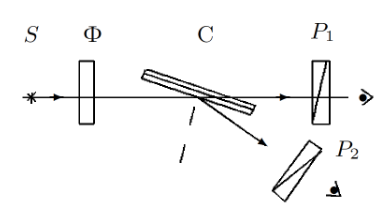
\includegraphics[width=0.4\linewidth]{img5.png}
\caption{Исследование стопы}
\label{img5}
\end{figure}

Посмотрели через поляроид $P_1$ на преломленный луч, он виден относительно четко. Затем посмотрели на отраженный луч, его увидели намного тусклее.

\subsection{Определение главных направлений двоякопреломляющих пластин}

\begin{enumerate}
    \item Поставили однородную кристаллическую пластинку между скрещёнными поляроидами $P_1$ и $P_2$.
    
    \begin{figure}[h]
    \centering
    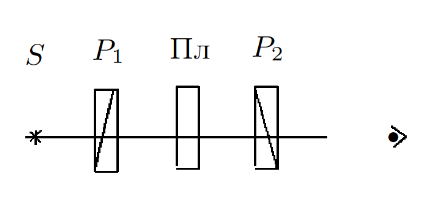
\includegraphics[width=0.4\linewidth]{img6.png}
    \caption{Определение главных направлений в пластинках}
    \label{img6}
    \end{figure}
    
    \item Вращая пластинку вокруг направления, наблюдая за интенсивностью света, проходящего сквозь второй поляроид, определили, что главные направления пластинки совпадают с разрешёнными направлениями поляроидов при условии, что вектор $\mathbf{E}$ спроецирован на быстрые и медленные направления за счёт поворота поляроида на угол порядка $\approx45$ градусов относительно минимума.
    
    \item Повторили опыт для второй пластинки, результат тот же
\end{enumerate}

\subsection{Выделение пластин $\lambda/2$ и $\lambda/4$}

\begin{enumerate}
    \item Добавили к схеме зелёный светофильтр; установили разрешённое направление поляроида горизонтально, а главные главные направления исследуемой пластинки -- под углом $45$ градусов к горизонтали.
    
    \item Смотря через поляроид $P_2$ на пластинку, вращаем поляроид. Если интенсивность лучей падает незначительно, то это означает, что свет имеет круговую поляризацию на выходе из пластинки. Значит это пластинка $\lambda/4$, которая изменяет фазовую характеристику волны на $\pi/2$.

    \item Если же интенсивность лучей заметно падает при вращении поляроида, мы можем различить минимум и максимум, то это означает, что свет на выходе из пластинки поляризован линейно. Значит это пластинка $\lambda/2$, которая изменяет фазовую характеристику волны на $\pi$.
\end{enumerate}

\subsection{Определение "быстрой" и "медленной" оси в пластинке $\lambda/4$}
\begin{enumerate}
    \item Поставили между скрещёнными поляроидами пластинку чувствительного оттенка ($\lambda$ для зелёного света), имеющую вид стрелки. Световой вектор, ориентированный вдоль направления стрелки, проходит с большей скоростью, перпендикулярный -- с меньшей.
    
    Установили разрешённое направление первого поляроида горизонтально, второй поляроид скрестили с первым. Поставили между ними фильтр и пластинку чувствительного оттенка, наблюдаем минимум через второй поляроид. Когда мы убираем пластинку, минимум сохранялся, а это значит, что эта пластинка не меняет поляризацию зелёного света в условиях предыдущего опыта.

    \item Убрали зелёный фильтр и поставили между скрещёнными поляроидами пластинку $\lambda$. Глядя сквозь второй поляроид на стрелку, убедились, что она имеет пурпурный цвет. Это происходит из-за того, что зелёный свет задерживается вторым поляроидом (изначально поляроиды были скрещены для длины волны зелёного света), а красная и синяя компоненты проходят.

    \item Добавили к схеме пластинку $\lambda/4$, главные направления которой совпадают с главными направлениями пластины $\lambda$ и ориентированы под углом $45$ градусов к разрешённым направлениям скрещённых поляроидов.
    
    При повороте рейтера со стрелкой на $180$ градусов вокруг вертикальной оси цвет стрелки меняется от зелёно-голубого до оранжево-жёлтого. Дело в том, что в зависимости от того, совпадают или не совпадают быстрые оси поляроидов, совокупность пластинок даёт либо $3\pi/4$, либо $5\pi/4$, что соответствует жёлтому и синему цветовым оттенкам. 
\end{enumerate}

\subsection{Интерференция поляризованных лучей}

Раслоположим между скрещенными поляроидами мозаичную слюдяную пластинку. Она собрана из 4-х узких полосок слюды, лежащих по сторонам квадрата (две полоски $\lambda/4$ и по одной - $\lambda/2$ и $3\lambda/4$). В центральном квадратике слюды нет. Главные направления свех пластинок ориентированы параллельно сторонам квадрата.

\begin{enumerate}
    \item Вращая пластинку, наблюдаем за изменениями цвета или интенсивности в отдельном квадратике.

    Разные квадратики пластинки имеют разную "толщину" и при повороте пластинки проходящий свет через пластинку поляризуется по разному, в результате чего цвет или интенсивность меняются в отдельных квадратиках.

    \item Теперь, не трогая пластинки, вращаем второй поляроид.

    Вращая поляроид, мы изменяем тип поляризации, в результате чего свет на выходе из пластинки поляризуется по разному, происходит так же смена цвета, поэтому при вращении цвет периодически переходит из ярких оттенков в прозрачные.
\end{enumerate}

\subsection{Определение направления вращения светового вектора в эллиптически поляризованной волне}

\begin{enumerate}
    \item Нарисуем эллипс поляризации для вектора $\mathbf{E}$, вышедшего из пластинки $\lambda/4$, и укажем на нём направления большей и меньшей скорости. Рядом нарисуем две вышедших из пластинки синусоиды: $x(t)$ и $y(t)$ со сдвигом фаз в четверть периода.

    \item Снова поставим между скрещенными поляроидами зеленый фильтр, а за ним - пластинку произвольной толщины

    \item Получили эллиптически-поляризованный свет. Для этого установили разрешенное направление первого поляроида под углом 10-20 градусов к горизонтали. Установили разрешенное направление второго поляроида вертикально и, вращая пластинку, нашли минимальную интенсивность света, прошедшего второй поляроид. Вращая второй поляроид убедились, что свет поляризован эллиптически.

    Таким образом, мы получили эллипс поляризации с вертикально ориентированной малой осью.
    
    \begin{figure}[h]
    \begin{center}
        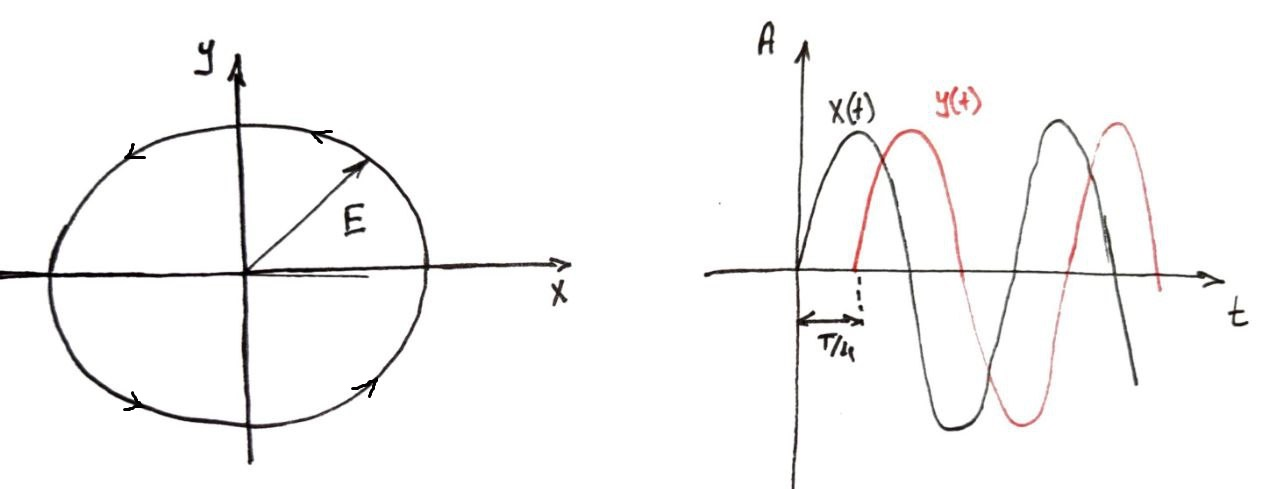
\includegraphics[width=0.9\linewidth]{img4.jpg}
    \end{center}
        \caption{Эллипс поляризациидля вектора $\mathbf{E}$, вышедшего из пластинки $\lambda/4$}
        \label{img9}
    \end{figure}

    \item Для определения направления вращения светового вектора в эллипсе установили между поляроидами дополнительную пластинку $\lambda/4$ с известными направлениями "быстрой" и "медленной" осей, ориентированными по осям эллипса поляризации анализируемого света. В этом случае вектор $\mathbf{E}$ на выходе будет таким, как если бы свет прошёл две пластинки $\lambda/4$: в совокупности они дают пластинку $\lambda/2$ или $0\cdot\lambda$, которая линейно поляризует свет.

    То есть, пластинки по одиночке дают эллипсы, вращающиеся в разные стороны, но поставленные друг за другом, они скомпенсируют разность фаз.

\end{enumerate}

\section{Выводы}
В данной лабораторной работе мы изучали поляризованный свет, поставили серию экспериментов, по результатам которых:
\begin{enumerate}
    \item определили разрешённые направления поляроидов
    \item определили угол Брюстера для эбонита
    \item исследовали стопу Столетова
    \item определили главные плоскости двоякопреломляющих пластин
    \item научились различать пластинки $\lambda/4$ и $\lambda/2$ как поляризоторы
    \item определили направление большей и меньшей скорости в пластинке $\lambda/4$
    \item исследовали интерференцию поляризованных лучей
    \item исследовали направления вращения светового вектора в эллиптически поляризованной волне.
\end{enumerate}

Наблюдаемые явления полностью согласуются с теоретическими выкладками, что говорит о точности проведения данных экспериментов.

\end{document}
